\def\longueurVecteurs{1.75}
\def\interSpace{1.5}
\def\interSpaceY{6}

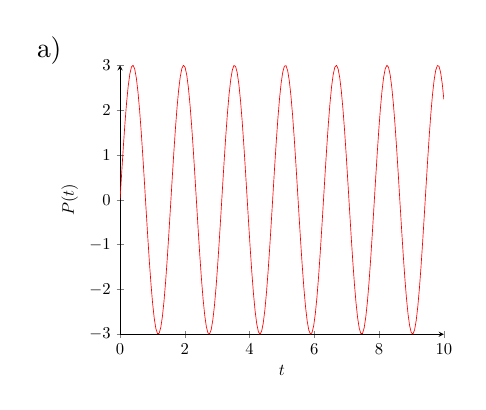
\begin{tikzpicture}[scale=0.6]
  %\tikzstyle{fleche}=[->,>=stealth];
  \draw (-\interSpace, \interSpaceY) node {{a)}};
  \begin{axis}[
    axis lines = left,
    xlabel = \(t\),
    ylabel = {\(P(t)\)},
]
\addplot [
    domain=0:10, 
    samples=200, 
    color=red,
]
{3*sin(deg(4*x))};

\end{axis}
\end{tikzpicture}
\begin{tikzpicture}[scale=0.6]
  %\tikzstyle{fleche}=[->,>=stealth];
  \draw (-\interSpace, \interSpaceY) node {{b)}};
  \begin{axis}[
    axis lines = left,
    xlabel = \(t\),
    ylabel = {\(P(t)\)},
]
\addplot [
    domain=0:10, 
    samples=200, 
    color=red,
]
{2*exp(-x)*cos(deg(4*x))};

\end{axis}
\end{tikzpicture}

\begin{tikzpicture}[scale=0.6]
  %\tikzstyle{fleche}=[->,>=stealth];
  \draw (-\interSpace, \interSpaceY) node {{c)}};
  \begin{axis}[
    axis lines = left,
    xlabel = \(t\),
    ylabel = {\(P(t)\)},
]
\addplot [
    domain=0:10, 
    samples=200, 
    color=red,
]
{2*exp(-x)*sin(deg(4*x))};

\end{axis}
\end{tikzpicture}
\begin{tikzpicture}[scale=0.6]
  %\tikzstyle{fleche}=[->,>=stealth];
  \draw (-\interSpace, \interSpaceY) node {{d)}};
  \begin{axis}[
    axis lines = left,
    xlabel = \(t\),
    ylabel = {\(P(t)\)},
]
\addplot [
    domain=0:10, 
    samples=200, 
    color=red,
]
{3*exp(-x)*cos(deg(4*x))};

\end{axis}
\end{tikzpicture}
